\documentclass[a4paper,oneside]{article}
%Compilé avec MacTex
\usepackage[french]{babel}
\usepackage[utf8]{inputenc}
\usepackage{hyperref} % références dans pdf
\usepackage[tt]{titlepic}
\usepackage{graphicx} % pour images
\usepackage{rotating} % pour rotatebox
\usepackage{lmodern}
\usepackage{amsmath}
\usepackage{amssymb}
\usepackage{mathrsfs}
\usepackage{sistyle}
\usepackage{chngpage}
\usepackage{epstopdf}
\usepackage{gnuplottex}% pour faire du gnuplot directement dans le latex
\usepackage[nottoc, notlof, notlot]{tocbibind} % pour que bibliographie soit comprise comme un chapitre ou section
\usepackage{appendix} % pour les annexes
\pagestyle{headings} % pour en têtes
\usepackage{mathenv}
\DeclareTextSymbol{\degre}{OT1}{23} %pour le symbole degré
\makeatletter % pour /bigcenter qui permet de s'affranchir des marges pour les images
\newskip\@bigflushglue \@bigflushglue = -100pt plus 1fil

\def\bigcenter{\trivlist \bigcentering\item\relax}
\def\bigcentering{\let\\\@centercr\rightskip\@bigflushglue%
\leftskip\@bigflushglue
\parindent\z@\parfillskip\z@skip}
\def\endbigcenter{\endtrivlist}
\makeatother


\begin{document}

%************************************************************************
%									TITRE
%************************************************************************


\begin{titlepage} % Suppresses headers and footers on the title page

	\centering % Centre everything on the title page

	\scshape % Use small caps for all text on the title page

	\vspace*{\baselineskip} % White space at the top of the page


	\rule{\textwidth}{1.6pt}\vspace*{-\baselineskip}\vspace*{2pt}
	 % Thick horizontal rule
	\rule{\textwidth}{0.4pt} % Thin horizontal rule

	\vspace{0.75\baselineskip} % Whitespace above the title

	{\LARGE RAPPORT DE VALIDATION :\\
	\vspace{0.75\baselineskip}
	Simulation de Lois Probabilistes \\
	} % Title

	\vspace{1\baselineskip} % Whitespace below the title
	\rule{\textwidth}{0.4pt}\vspace*{-\baselineskip}\vspace*{3.2pt}
	 % Thin horizontal rule
	\rule{\textwidth}{1.6pt} % Thick horizontal rule
	\vspace{2\baselineskip} % Whitespace after the title block

	%------------------------------------------------
	%	Subtitle
	%------------------------------------------------

	% Subtitle or further description
	Probabilités - Statistiques

	\vspace*{3\baselineskip} % Whitespace under the subtitle

	%------------------------------------------------
	%	Editor(s)
	%------------------------------------------------


	\vspace{0.5\baselineskip} % Whitespace before the editors

	{\scshape\Large Quentin Bergé \\} % Editor list

	\vspace{0.5\baselineskip} % Whitespace below the editor list

	\textit{ENSEEIHT} % Editor affiliation

	\vfill % Whitespace between editor names and publisher logo

	%------------------------------------------------
	%	Publisher
	%------------------------------------------------

	
\includegraphics[scale=0.8]{logoN7.png} % changer logo

	\vspace{0.3\baselineskip} % Whitespace under the publisher logo

Avril 2019 % Publication year
\end{titlepage}
\newpage

%Table des Matières
\tableofcontents
\newpage

%*******************************************************
% 						DEBUT RAPPORT
%********************************************************

\section{Introduction}

L'objet de ce court rapport est de rendre compte des travaux effectués avec Matlab dans le cadre de simulation des principales lois probabilistes.

\section{Variables Continues}

\subsection{Génération et Simulation de la loi Uniforme}

L'objet de cet exercice était de comparer la génération d'une loi uniforme selon la méthode de l'histogramme des fréquences normalisées et le générateur natif de Matlab rand.

On a effectué la génération pour $10^3$ et $10^7$ échantillons.  

\begin{figure}[h]
    \begin{minipage}[c]{.46\linewidth}
        \centering
        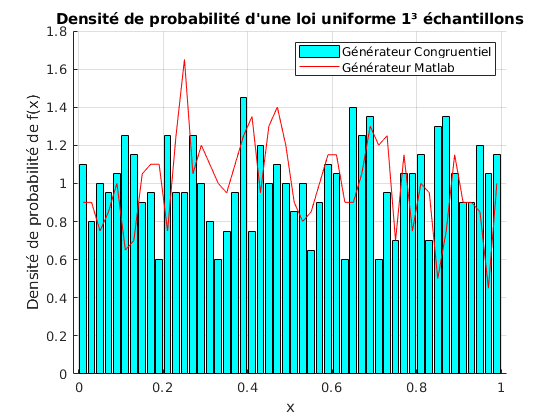
\includegraphics[scale=0.5]{../Exercice1/N=1000.png}
        \caption{$10^3$ échantillons}
    \end{minipage}
    \hfill%
    \begin{minipage}[c]{.46\linewidth}
        \centering
        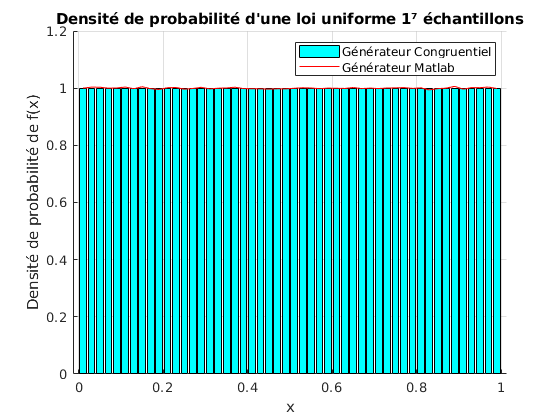
\includegraphics[scale=0.5]{../Exercice1/N=10000000.png}
        \caption{$10^7$ échantillons}
    \end{minipage}
\end{figure}

On constate que lorsqu'on augmente le nombre d'échantillons, on se rapproche du résultat attendu, c'est à dire la densité de probabilité d'une loi uniforme centrée réduite. On observe bien ceci dans le cas de $10^7$ échantillons.

Le résultat obtenu avec la méthode de l'histogramme des fréquences normalisées est alors celui attendu. 

\newpage
\subsection{Simulation d'une Loi Gaussienne}

\subsubsection{Partie 1 : Fonction randn de Matlab}

On générera ici le vecteur gaussien à l'aide de la fonction \verb?randn?.

Dans cette partie, l'objectif est de comparer les méthodes :
\begin{itemize}
	\item histogramme des fréquences normalisés notée \verb?ddp?
	\item normpdf notée \verb?normpdf?
	\item densité de probabilité d'une loi normale notée \verb?fx2?
\end{itemize}


\begin{figure}[h!]
\centering
    \begin{minipage}[c]{.46\linewidth}
        \centering
        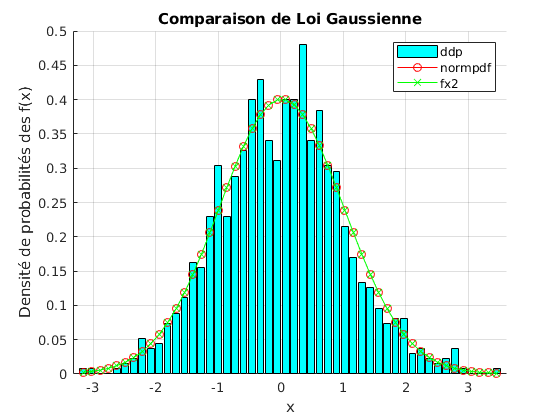
\includegraphics[scale=0.5]{../Exercice2/Part1N=1000.png}
        \caption{$10^3$ échantillons}
    \end{minipage}
    \hfill%
    \begin{minipage}[c]{.46\linewidth}
        \centering
        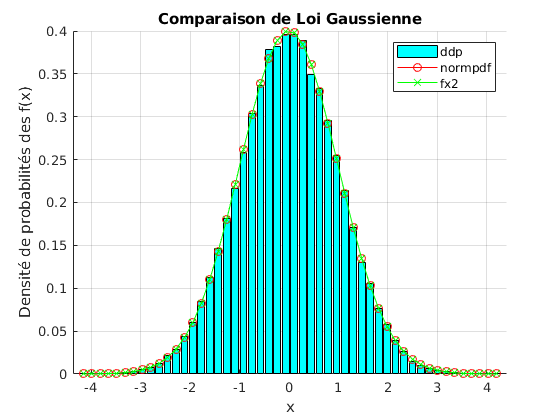
\includegraphics[scale=0.5]{../Exercice2/Part1N=100000.png}
        \caption{$10^5$ échantillons}
    \end{minipage}
\end{figure}

On constate qu'on obtient bien le résultat attendu c'est à dire une loi gaussienne centrée en 0. Néanmoins on constate que les méthodes normpdf et la densité de probabilité d'une loi normale donnent de bien meilleurs résultats avec moins d'échantillons que la méthode de l'histogramme des fréquences normalisées

\newpage
\subsubsection{Partie 2 : Méthode de Box Muller}
Dans cette partie on souhaite simuler la loi gaussienne avec la méthode de Box Muller.

\begin{figure}[h]
\centering
    \begin{minipage}[c]{.46\linewidth}
        \centering
        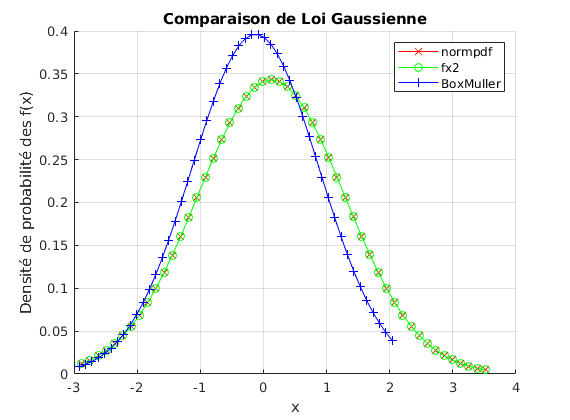
\includegraphics[scale=0.5]{../Exercice2/BMN=100.png}
        \caption{$10^2$ échantillons}
    \end{minipage}
    \hfill%
    \begin{minipage}[c]{.46\linewidth}
        \centering
        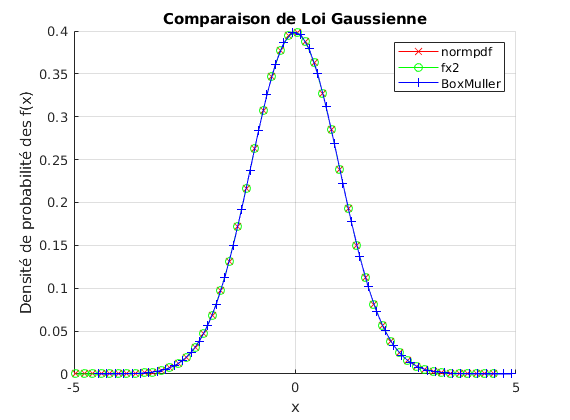
\includegraphics[scale=0.5]{../Exercice2/BMN=1E6.png}
        \caption{$10^6$ échantillons}
    \end{minipage}
\end{figure}
 

 On peut remarquer que la méthode de Box Muller semble converger plus rapidement, c'est à dire avec moins d'échantillons, vers le résultat final.
 
 
 \begin{center}
 \begin{tabular}{|c|c|c|}
 
 	\hline
 	échantillons & $10^3$ & $10^6$\\
 	\hline
 	$mx_{BM}$ & 0.0106 & 0.0018 \\ 
 	$sx_{BM}$ & 1.0016 & 0.99995 \\
 	$mx$ & 0.0024 & $5.10^{-4}$ \\
 	$sx$ & 0.9998 & 1.0004 \\
 	\hline
 	
 \end{tabular}
  \end{center}
  	
Ce dernier tableau confirme bien que les moyennes et les écarts-types valent bien respectivement 0 et 1.

\newpage

 \subsection{Simulation d'une Loi Exponentielle}
 Dans cet exercice, nous allons comparer la simulation d'une loi exponentielle avec les méthodes de l'histogramme des fréquences normalisées et de la densité de probabilité d'une loi exponentielle.
 Tout d'abord nous affichons uniquement l'histogramme des fréquences normalisées.
 
 \begin{figure}[h!]
\centering
    \begin{minipage}[c]{.46\linewidth}
        \centering
        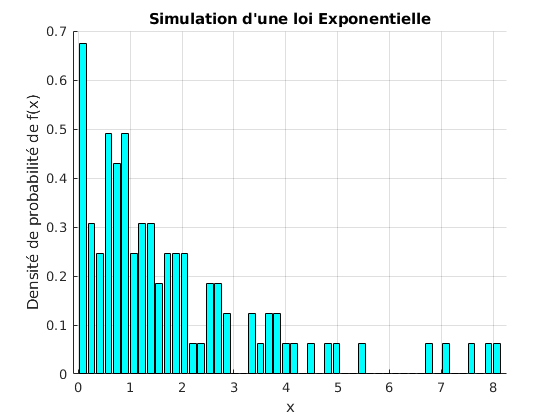
\includegraphics[scale=0.5]{../Exercice3/ddpN=100.png}
        \caption{$10^2$ échantillons}
    \end{minipage}
    \hfill%
    \begin{minipage}[c]{.46\linewidth}
        \centering
        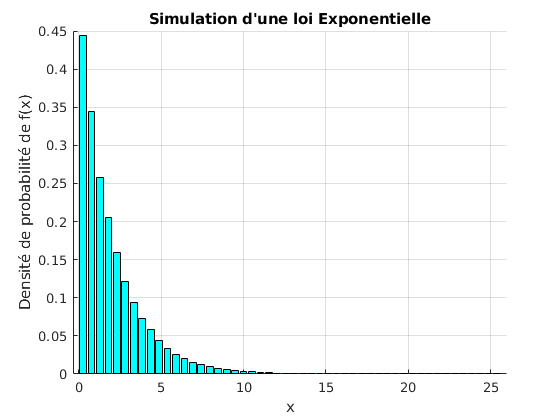
\includegraphics[scale=0.5]{../Exercice3/ddpN=100000.png}
        \caption{$10^5$ échantillons}
    \end{minipage}
\end{figure}
 

 Puis nous comparons les 2 méthodes :
 
 \begin{figure}[h!]
\centering
    \begin{minipage}[c]{.46\linewidth}
        \centering
        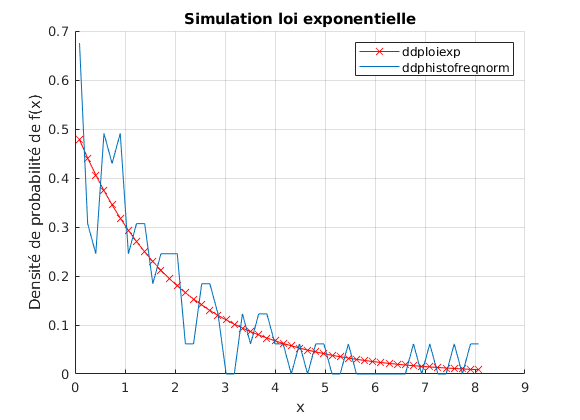
\includegraphics[scale=0.5]{../Exercice3/Part2N=100.png}
        \caption{$10^2$ échantillons}
    \end{minipage}
    \hfill%
    \begin{minipage}[c]{.46\linewidth}
        \centering
        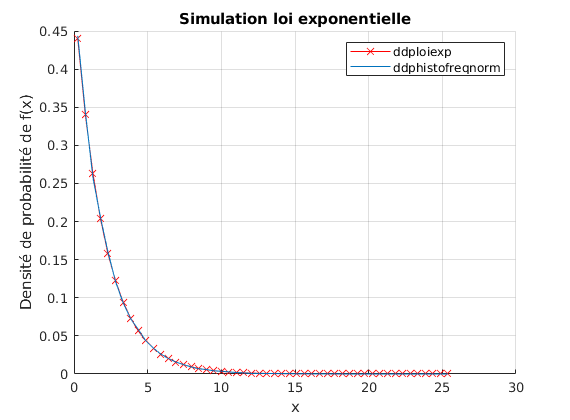
\includegraphics[scale=0.5]{../Exercice3/Part2N=100000.png}
        \caption{$10^6$ échantillons}
    \end{minipage}
\end{figure}

On peut observer que la densité de probabilité notée \verb?ddploiexp? donne de meilleurs résultats dès $100$ échantillons tandis que la méthode de l'histogramme des fréquences normalisées notée \verb?ddphistofreqnorm? nécéssite $10^5$ échantillons pour donner de bons résultats.

\newpage
\subsection{Simulation d'une Loi de Bernouilli}

Il s'agit ici de représenter une loi de Bernouilli.

 \begin{center}
\begin{tabular}{|c|c|c|c|c|}
 
\hline
 	échantillons & 10 & 100 & $10^3$ & $10^6$\\
 	\hline
 	$P(A)$ & 0.7 & 0.78 & 0.7960 & 0.79989 \\ 
 	
 	\hline
 	\end{tabular}
 	\end{center}
 	
 On observe bien que plus on augmente le nombre d'échantillons, plus on se rapproche de la probabilité de succès qui est de $0.8$.	
 
 \section{Conclusion}
 
Nous avons pu nous rendre compte de l'utilité de Matlab pour effectuer des simulations de loi probabiliste.
 
\end{document}